\chapter[Resultados]{Resultados e Discussões}
\label{ch:resultados}
% TER EM MENTE:
% Refere-se à apresentação em ordem lógica dos resultados obtidos, sem interpretação pessoal do autor. Devem ser apresentados de forma objetiva, precisa e lógica, utilizando tabelas, gráficos, figuras etc.

% APENAS PARA ILUSTRAR O TIPO DE PLOTS QUE PRETENDO COLOCAR
% CONSIGO REFAZER QUALQUER PLOT FACILMENTE
% TENHO INFORMAÇÃO/DADOS PARA GERAR DIVERSOS PLOTS E TESTES OFFLINE

% OBJETIVO:
% 1) MOSTRAR O RESULTADO DA CALIBRAÇÃO (CURVA ESTIMADA X DADOS BRUTOS)
% 2) MOSTRAR O RESULTADO DA FILTRAGEM; COMPARAR COM FILTOS SIMPLES (POSSO APLICAR OS FILTROS OFFLINE NOS DADOS COLETADOS)
% 3) MOSTRAR O RESULTADO DO CONTROLE, PRINCIPALMENTE COM O INTUITO DE DIMINUIR AS ASSIMETRIAS DOS MOTORES

% MOSTRAR:
% RESPOSTAS PARA DIFERENTES CONFIGURAÇÕES DE MOTOR-SENTIDO E COM DIFERENTES REFERENCIAS/SINAIS DE CONTROLE PARA:
% CURVA ESTIMADA X SEM FILTRO X COM FILTRO
% \section{Resultados da calibração}

% Please add the following required packages to your document preamble:
% \usepackage{graphicx}
\begin{table}[H]
\centering
\resizebox{\textwidth}{!}{%
\begin{tabular}{c|cc|cc|cc|cc}
\multicolumn{1}{r|}{\textbf{}} &
  \multicolumn{2}{c|}{\textbf{$K_m$ {[}rad/s{]}}} &
  \multicolumn{2}{c}{\textbf{$\tau_m$ {[}s{]}}} &
  \multicolumn{2}{c|}{\textbf{$K_p$ {[}$1/(rad/s)${]}}} \\
\textbf{Experimento} &
  \textbf{\begin{tabular}[c]{@{}c@{}}Motor\\ Esquerdo\end{tabular}} &
  \textbf{\begin{tabular}[c]{@{}c@{}}Motor\\ Direito\end{tabular}} &
  \textbf{\begin{tabular}[c]{@{}c@{}}Motor\\ Esquerdo\end{tabular}} &
  \textbf{\begin{tabular}[c]{@{}c@{}}Motor\\ Direito\end{tabular}} &
  \textbf{\begin{tabular}[c]{@{}c@{}}Motor\\ Esquerdo\end{tabular}} &
  \textbf{\begin{tabular}[c]{@{}c@{}}Motor\\ Direito\end{tabular}} \\ \hline
\textbf{1} &
  3236.80 &
  3047.72 &
  7.62e-02 &
  6.57e-02 &
  1.37e-04 &
  1.24e-04 \\
\textbf{2} &
  4446.69 &
  4514.56 &
  5.71e-02 &
  5.40e-02 &
  3.01e-05 &
  3.23e-05 \\
\textbf{3} &
  4335.81 &
  4394.23 &
  5.48e-02 &
  5.30e-02 &
  1.54e-05 &
  2.11e-05 \\
\textbf{4} &
  3345.83 &
  3644.55 &
  4.43e-02 &
  5.90e-02 &
  5.55e-05 &
  3.80e-05
\end{tabular}%
}
\caption{Resultado da calibração para os diferentes experimentos.}
\label{tab:resumo_calibracao}
\end{table}

A Tabela \ref{tab:resumo_calibracao} contém, para os quatro experimentos e para cada motor, os resultados da calibração: Ganho da planta $K_m$; Constante de tempo $\tau_m$ e o ganho do controlador proporcional que foi calculado para se atingir o polo desejado $S_d = -20$ ($\tau_{d} = 0.08$ s) no experimento 1 e nos experimentos 2,3 e 4 foram usados $S_d = -10$ ($\tau_{d} = 0.05$ s).

\begin{figure}[H]
    % \centering
    \begin{subfigure}{.5\textwidth}
    \centering
    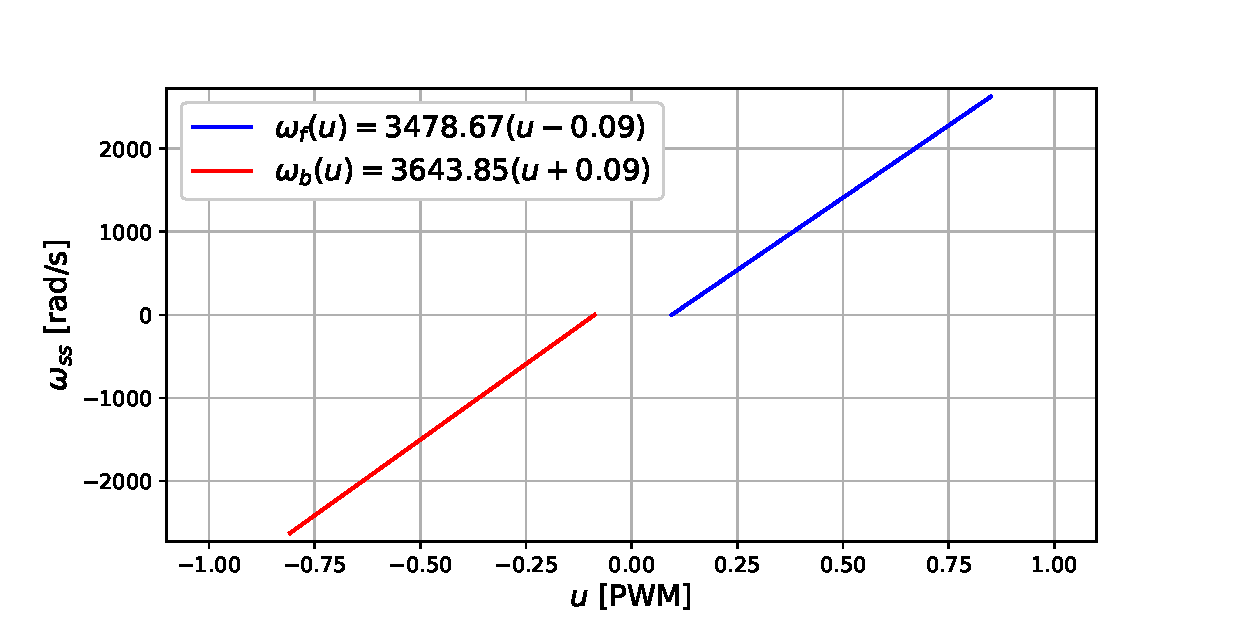
\includegraphics[width=\textwidth]{figuras/resultados/exp01/curva_feedforward_esquerdo100.eps}
    \caption{Curva $u(\omega)$ para o motor esquerdo.}
    \label{fig:exp01:curva_feedforward_esquerdo}
    \end{subfigure}
    \hfill
    \begin{subfigure}{.5\textwidth}
    \centering
    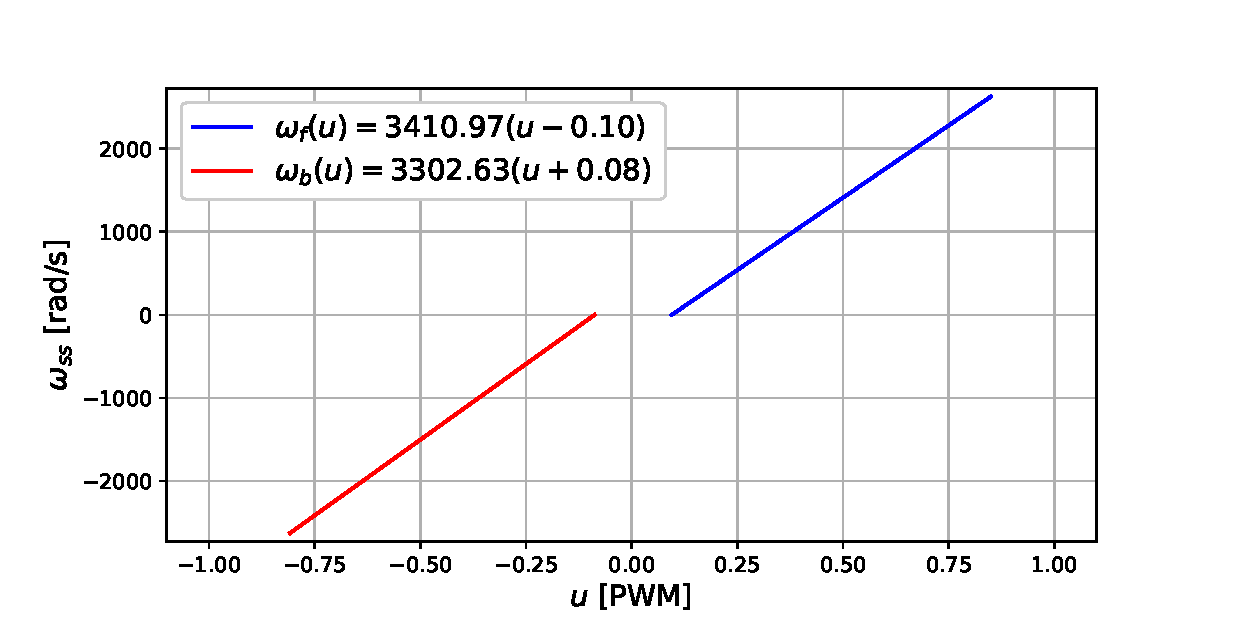
\includegraphics[width=\textwidth]{figuras/resultados/exp01/curva_feedforward_direito100.eps}
    \caption{Curva $u(\omega)$ para o motor direito.}
    \label{fig:exp01:curva_feedforward_direito}
    \end{subfigure}
    \begin{subfigure}{.5\textwidth}
    \centering
    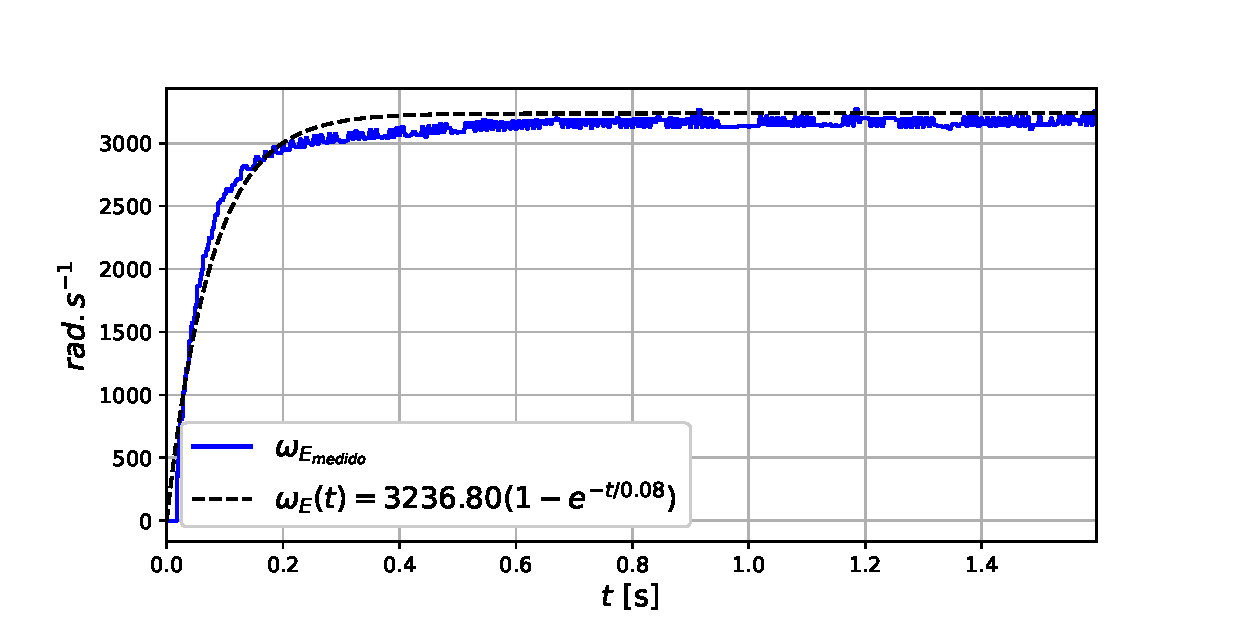
\includegraphics[width=\textwidth]{figuras/resultados/exp01/regressao_vs_medido_esquerdo100.eps}
    \caption{Curva $\omega(t)$ ideal, com os parâmetros da identificação vs velocidades medidas. Motor Esquerdo.}
    \label{fig:exp01:regressao_medido_esquerdo}
    \end{subfigure}
    \hfill
    \begin{subfigure}{.5\textwidth}
    \centering
    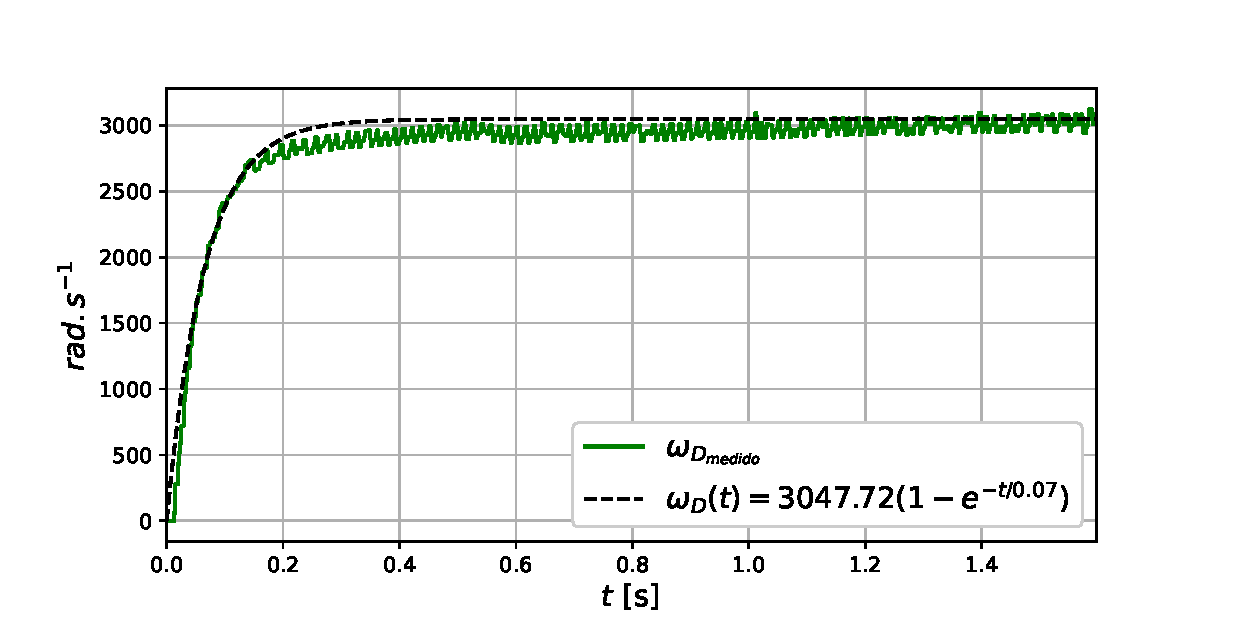
\includegraphics[width=\textwidth]{figuras/resultados/exp01/regressao_vs_medido_direito100.eps}
    \caption{Curva $\omega(t)$ ideal, com os parâmetros da identificação vs velocidades medidas. Motor Direito.}
    \label{fig:exp01:regressao_medido_direito}
    \end{subfigure}
    \hfill
    \begin{subfigure}{.5\textwidth}
    \centering
    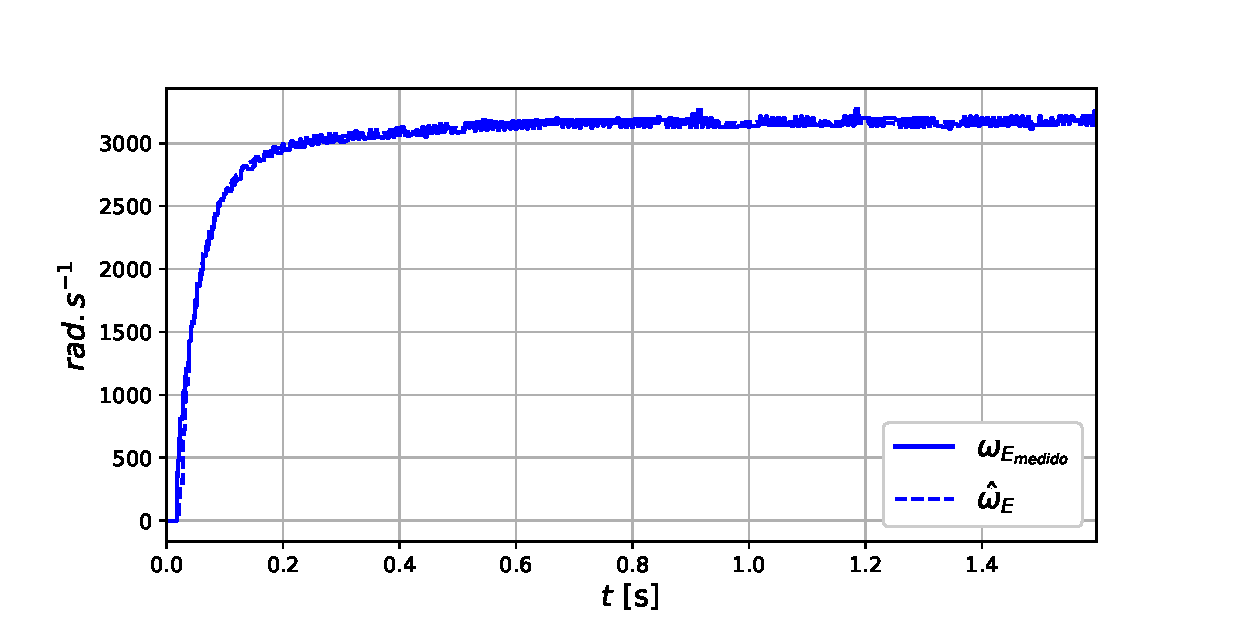
\includegraphics[width=\textwidth]{figuras/resultados/exp01/filtro_vs_sem_filtro_esquerdo100.eps}
    \caption{Comparação entre a velocidade estimativa $\hat{\omega}$ e a velocidade $\omega$ medida. Motor Esquerdo.}
    \label{fig:exp01:filtragem_esquerdo}
    \end{subfigure}
    \hfill
    \begin{subfigure}{.5\textwidth}
    \centering
    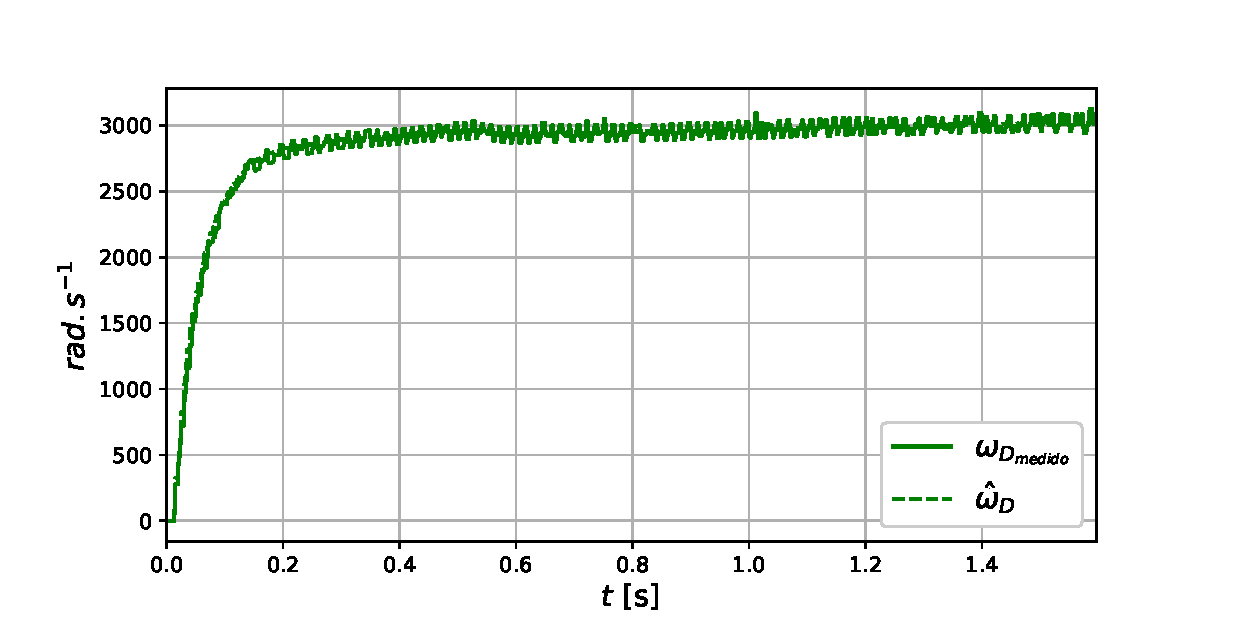
\includegraphics[width=\textwidth]{figuras/resultados/exp01/filtro_vs_sem_filtro_direito100.eps}
    \caption{Comparação entre a velocidade estimativa $\hat{\omega}$ e a velocidade $\omega$ medida. Motor Direito.}
    \label{fig:exp01:filtragem_direito}
    \end{subfigure}
    \hfill
    \begin{subfigure}{.5\textwidth}
    \centering
    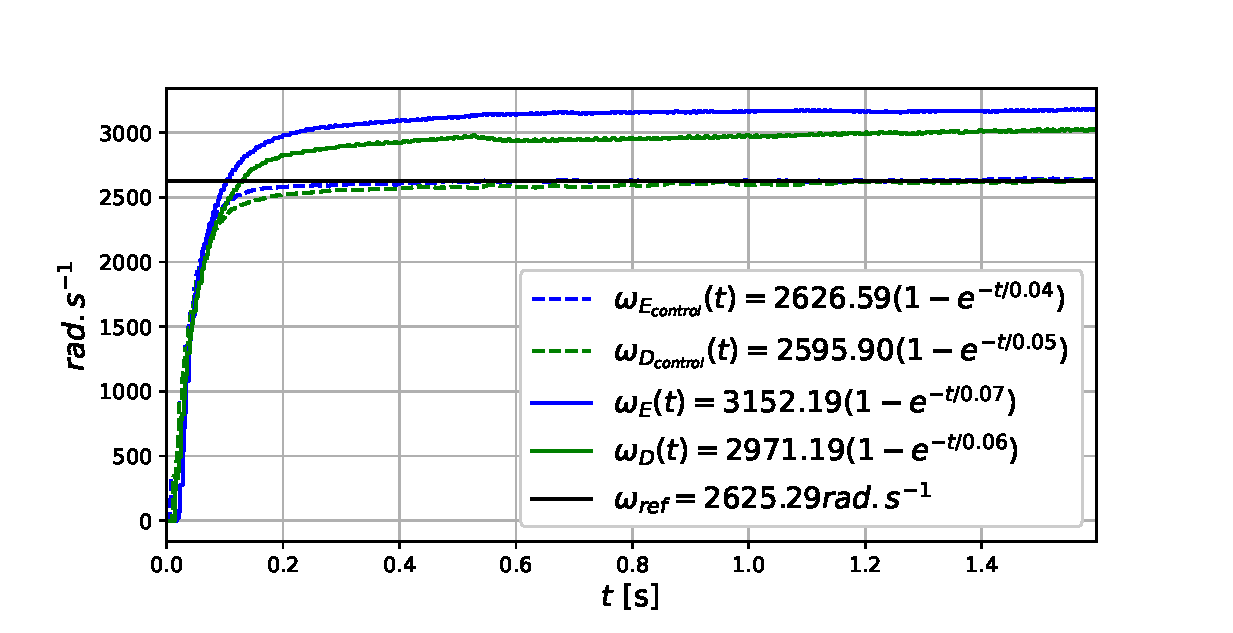
\includegraphics[width=\textwidth]{figuras/resultados/exp01/controlador_vs_sem_controlador100.eps}
    \caption{Comparação entre o sistema com controlador vs sem controlador.}
    \label{fig:exp01:controle}
    \end{subfigure}
    \hfill
    \begin{subfigure}{.5\textwidth}
    \centering
    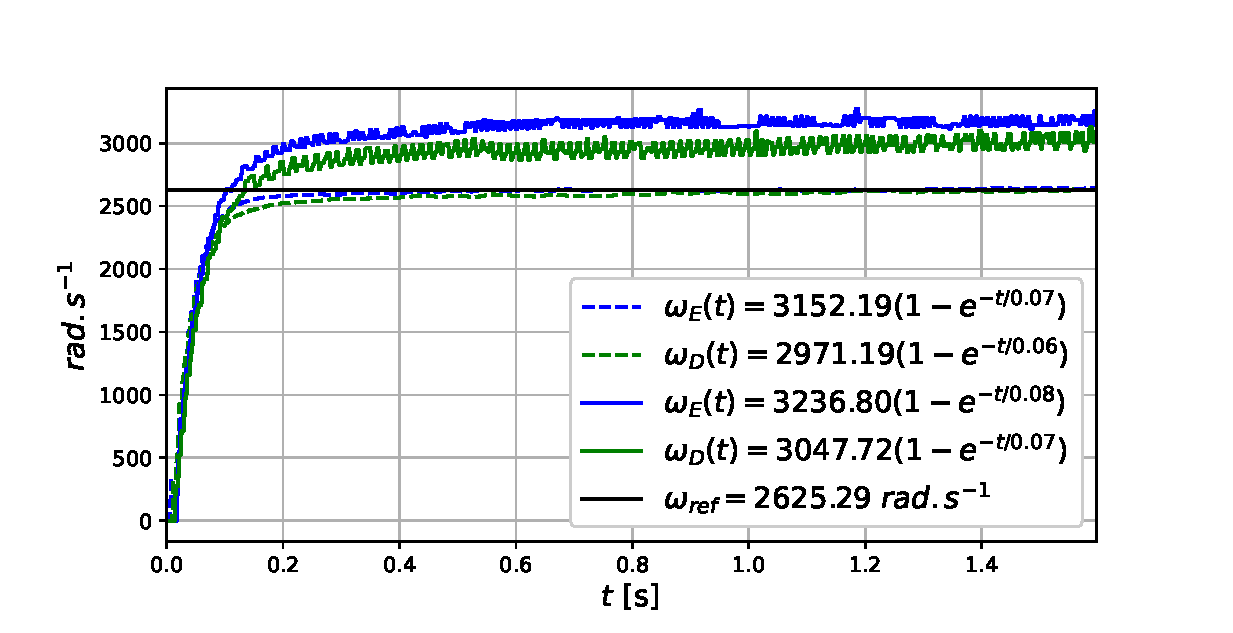
\includegraphics[width=\textwidth]{figuras/resultados/exp01/antes_vs_depois100.eps}
    \caption{Resposta sem observador e sem controle vs com controlador e observador.}
    \label{fig:exp01:antes_vs_depois}
    \end{subfigure}
    
    \caption{Experimento 1. \emph{Sinal de controle e Referência igual a 1.0.}}
    \label{fig:exp01_100}
\end{figure}


Os gráficos comparativos para o experimento 1 estão exibidos na Figura \ref{fig:exp01_100}. A partir dessas Figuras e da Tabela \ref{tab:resumo_calibracao} extraí-se que para o \textbf{Experimento 1}:

\begin{itemize}
    \item Analisando as Figuras \ref{fig:exp01:curva_feedforward_esquerdo} e \ref{fig:exp01:curva_feedforward_direito}:\\
        As zonas mortas ($|D|$) para o motor esquerdo e direito são respectivamente: $0.09$ (em ambos os sentidos de giro), 0.10 e 0.08 (na rotação que favorece o movimento para frente do robô e para trás, respectivamente).
    \item Pelas Figuras \ref{fig:exp01:regressao_medido_esquerdo} e \ref{fig:exp01:regressao_medido_direito}:\\
        Observa-se que a curva ideal (considerando o sistema de primeira ordem e com os parâmetros da calibração) apresenta um ganho levemente maior do que o que as medições aparentam para ambos os motores. E a constante de tempo aparenta corresponder bem ao observado pelas medições.
    \item Pelos gráficos das Figuras \ref{fig:exp01:filtragem_esquerdo} e \ref{fig:exp01:filtragem_direito} observa-se que:\\
        para ambos os motores a curva correspondente à velocidade $\hat{\omega}$ estimada pelo filtro, encontra-se sobrepondo-se a curva das velocidades medidas, porém, sem apresentar as mesmas oscilações (ruídos de quantização).
    \item Já pela Figura \ref{fig:exp01:controle} nota-se para ambos os motores:
        Que a resposta do sistema controlado está bem próximo da referência $\omega_{ref}$ e que a constante de tempo $\tau$ está como o desejado ($0.08s$).
    \item Por fim a Figura \ref{fig:exp01:antes_vs_depois} compara a resposta do sistema com o controlador+observador, com os mesmos sem estes. \\
        Nota-se que esse experimento apresenta naturalmente uma boa simetria na resposta de ambos os motores, apesar do motor direito apresentar um elevado erro de quantização. Mesmo assim, é possível observar que tanto a simetria é melhorada/mantida quanto o erro de quantização diminui significativamente para ambos os motores.
\end{itemize}

\begin{figure}[H]
    % \centering
    \begin{subfigure}{.5\textwidth}
    \centering
    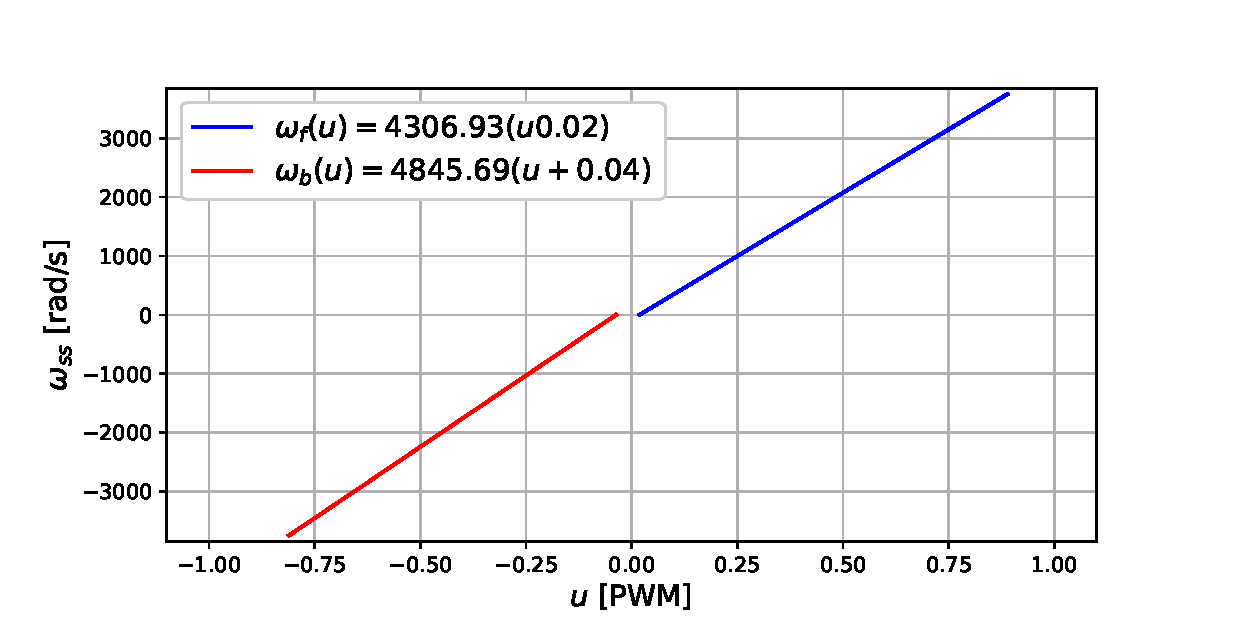
\includegraphics[width=\textwidth]{figuras/resultados/exp02/curva_feedforward_esquerdo100.eps}
    \caption{Curva $u(\omega)$ para o motor esquerdo.}
    \label{fig:exp02:curva_feedforward_esquerdo}
    \end{subfigure}
    \hfill
    \begin{subfigure}{.5\textwidth}
    \centering
    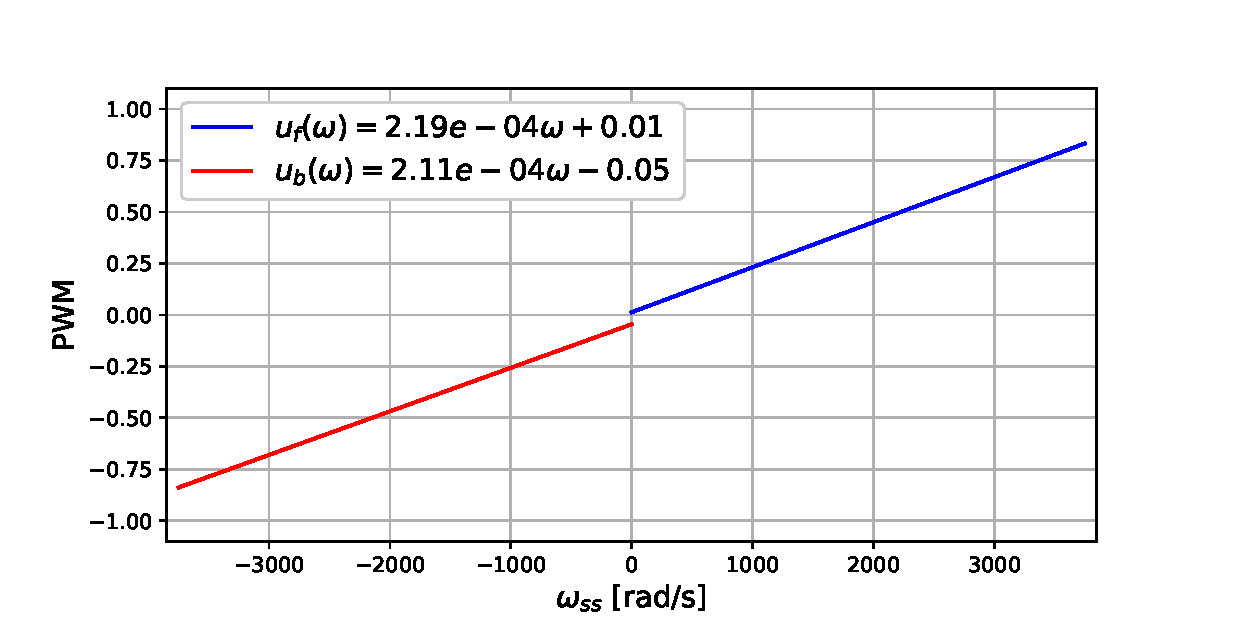
\includegraphics[width=\textwidth]{figuras/resultados/exp02/curva_feedforward_direito100.eps}
    \caption{Curva $u(\omega)$ para o motor direito.}
    \label{fig:exp02:curva_feedforward_direito}
    \end{subfigure}
    \begin{subfigure}{.5\textwidth}
    \centering
    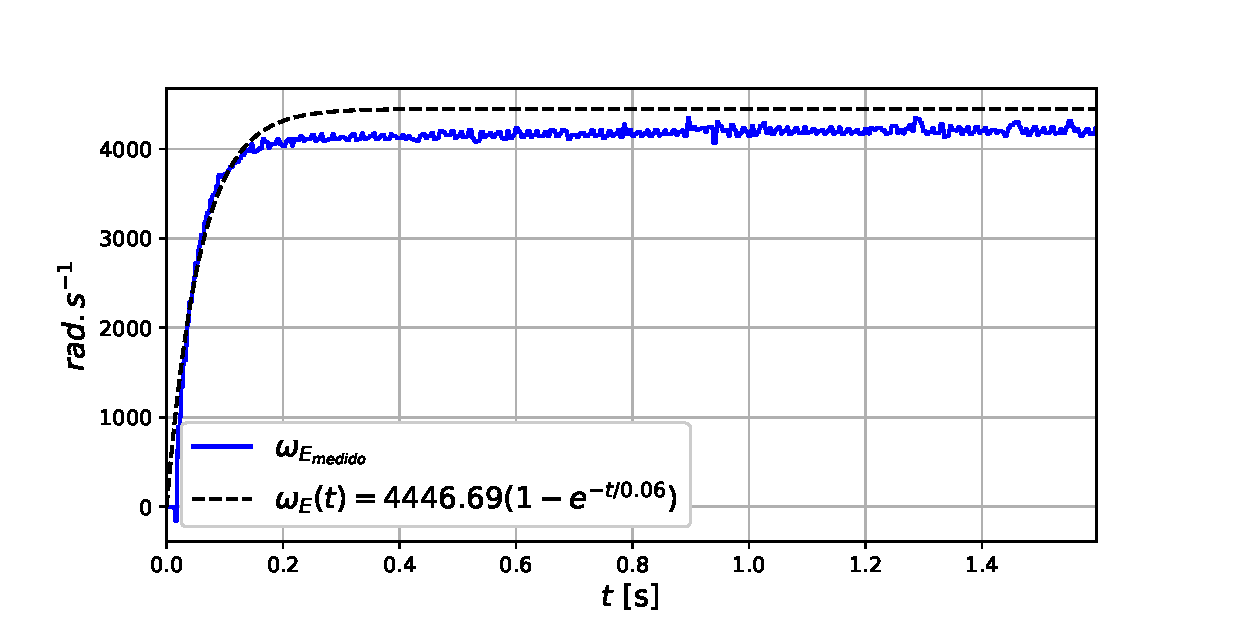
\includegraphics[width=\textwidth]{figuras/resultados/exp02/regressao_vs_medido_esquerdo100.eps}
    \caption{Curva $\omega(t)$ ideal, com os parâmetros da identificação vs velocidades medidas. Motor Esquerdo.}
    \label{fig:exp02:regressao_medido_esquerdo}
    \end{subfigure}
    \hfill
    \begin{subfigure}{.5\textwidth}
    \centering
    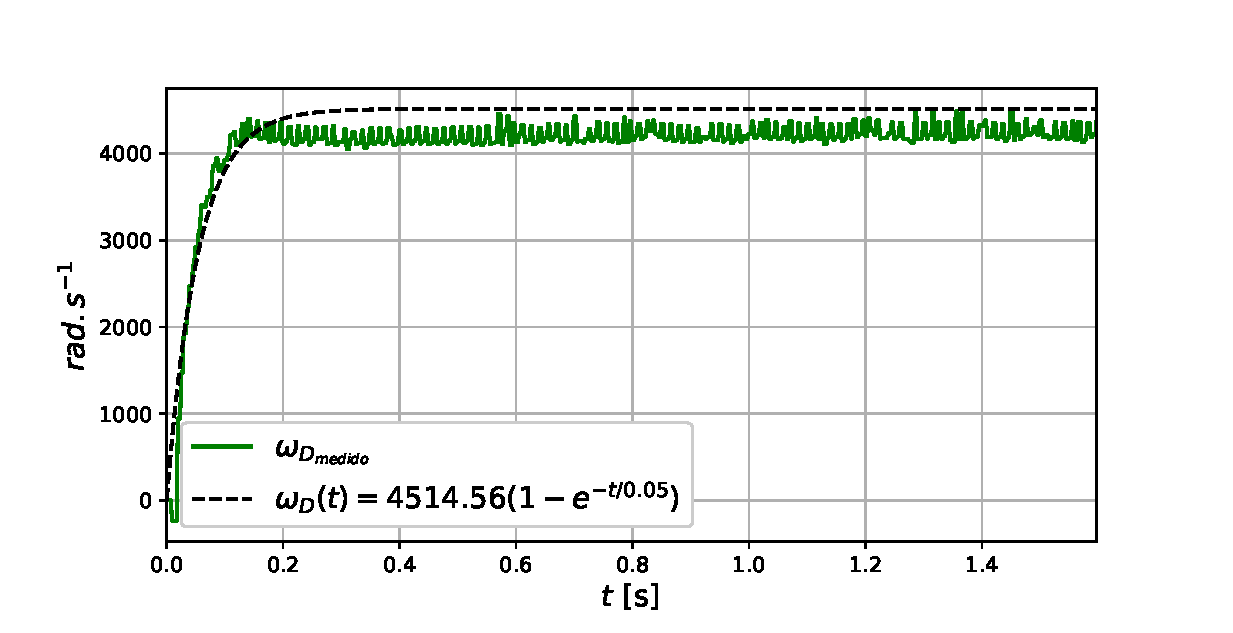
\includegraphics[width=\textwidth]{figuras/resultados/exp02/regressao_vs_medido_direito100.eps}
    \caption{Curva $\omega(t)$ ideal, com os parâmetros da identificação vs velocidades medidas. Motor Direito.}
    \label{fig:exp02:regressao_medido_direito}
    \end{subfigure}
    \hfill
    \begin{subfigure}{.5\textwidth}
    \centering
    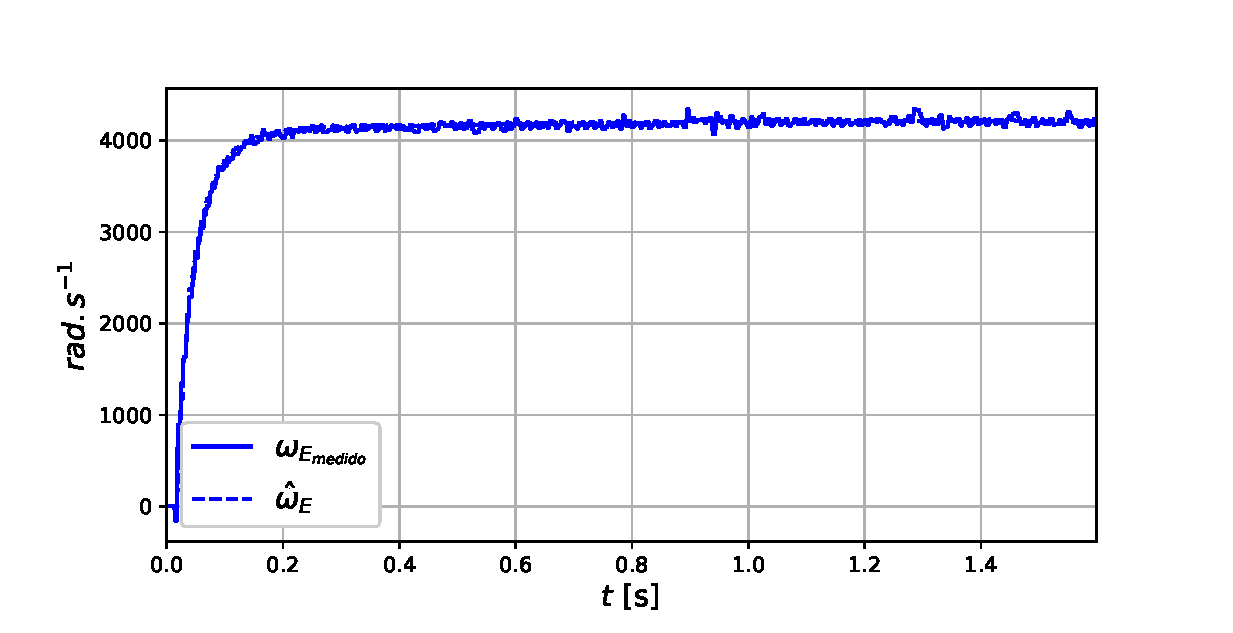
\includegraphics[width=\textwidth]{figuras/resultados/exp02/filtro_vs_sem_filtro_esquerdo100.eps}
    \caption{Comparação entre a velocidade estimativa $\hat{\omega}$ e a velocidade $\omega$ medida. Motor Esquerdo.}
    \label{fig:exp02:filtragem_esquerdo}
    \end{subfigure}
    \hfill
    \begin{subfigure}{.5\textwidth}
    \centering
    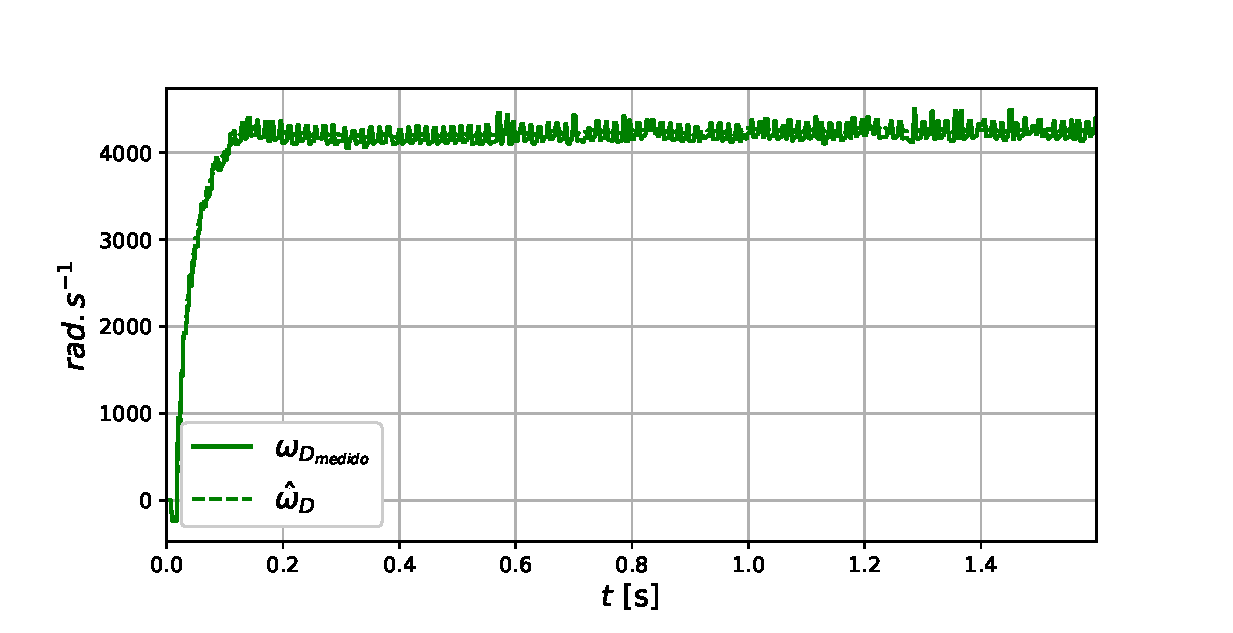
\includegraphics[width=\textwidth]{figuras/resultados/exp02/filtro_vs_sem_filtro_direito100.eps}
    \caption{Comparação entre a velocidade estimativa $\hat{\omega}$ e a velocidade $\omega$ medida. Motor Direito.}
    \label{fig:exp02:filtragem_direito}
    \end{subfigure}
    \hfill
    \begin{subfigure}{.5\textwidth}
    \centering
    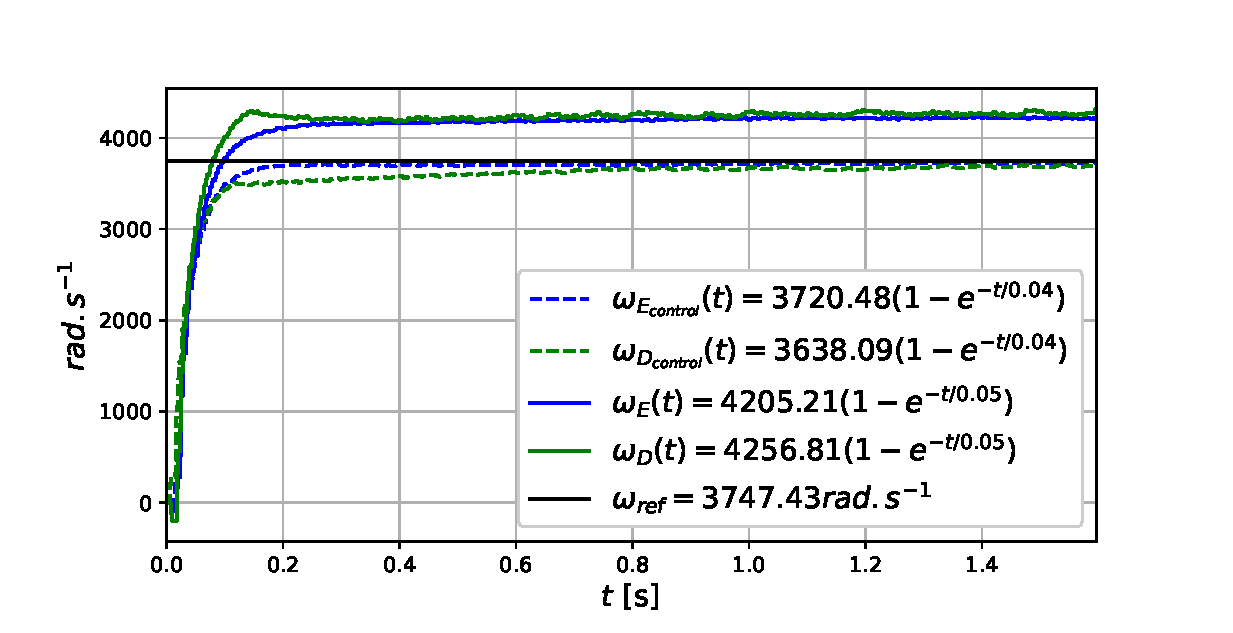
\includegraphics[width=\textwidth]{figuras/resultados/exp02/controlador_vs_sem_controlador100.eps}
    \caption{Comparação entre o sistema com controlador vs sem controlador.}
    \label{fig:exp02:controle}
    \end{subfigure}
    \hfill
    \begin{subfigure}{.5\textwidth}
    \centering
    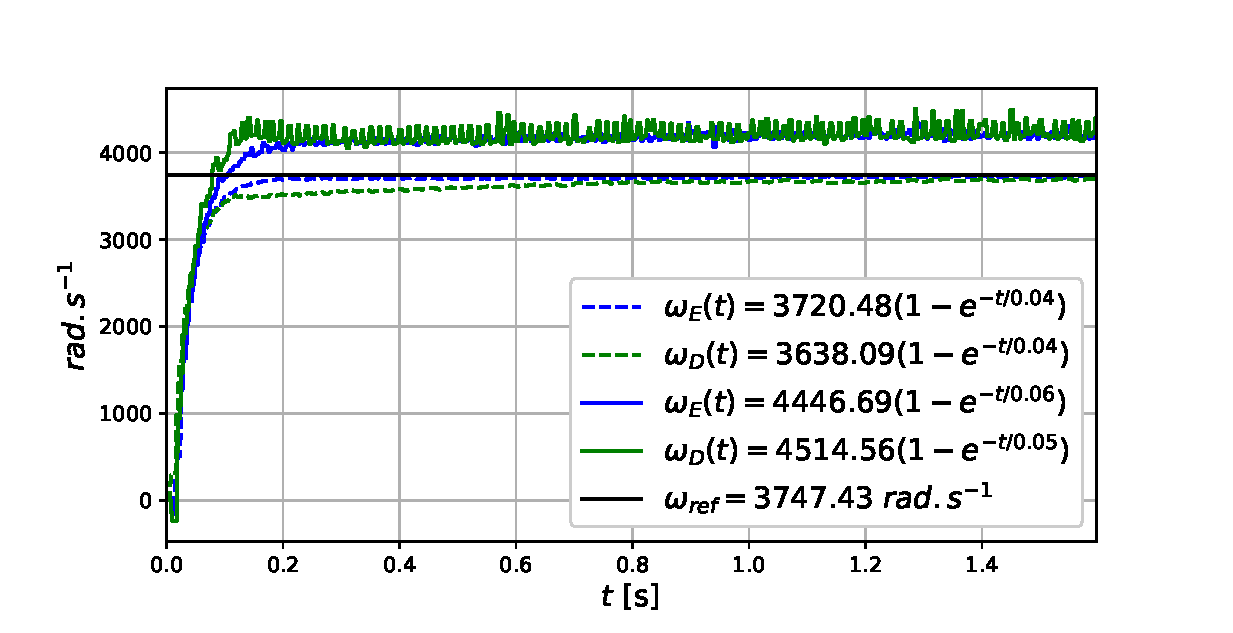
\includegraphics[width=\textwidth]{figuras/resultados/exp02/antes_vs_depois100.eps}
    \caption{Resposta sem observador e sem controle vs com controlador e observador.}
    \label{fig:exp02:antes_vs_depois}
    \end{subfigure}
    
    \caption{Experimento 2. \emph{Sinal de controle e Referência igual a 1.0.}}
    \label{fig:exp02_100}
\end{figure}

Os gráficos comparativos para o experimento 2 estão exibidos na Figura \ref{fig:exp02_100}. A partir dessas Figuras e da Tabela \ref{tab:resumo_calibracao} extraí-se que para o \textbf{Experimento 2}:

\begin{itemize}
    \item Analisando as Figuras \ref{fig:exp02:curva_feedforward_esquerdo} e \ref{fig:exp02:curva_feedforward_direito}:\\
        As zonas mortas ($|D|$) para o motor esquerdo e direito são respectivamente: $0.02$, $0.04$ (para frente e para trás, respectivamente), $0.01$ e $0.05$ (na rotação que favorece o movimento para frente do robô e para trás, respectivamente).
    \item Pelas Figuras \ref{fig:exp02:regressao_medido_esquerdo} e \ref{fig:exp02:regressao_medido_direito}:\\
        Observa-se que, assim como para o experimento 1, a curva ideal (considerando o sistema de primeira ordem e com os parâmetros da calibração) apresenta um ganho levemente maior do que o que as medições aparentam para ambos os motores. E a constante de tempo aparenta corresponder bem ao observado pelas medições.
    \item Pelos gráficos das Figuras \ref{fig:exp02:filtragem_esquerdo} e \ref{fig:exp02:filtragem_direito} observa-se que:\\
        para ambos os motores a curva correspondente à velocidade $\hat{\omega}$ estimada pelo filtro, encontra-se sobrepondo-se a curva das velocidades medidas, porém, sem apresentar o ruído de quantização.
    \item Já pela Figura \ref{fig:exp02:controle} nota-se para ambos os motores:
        Que a resposta do sistema controlado está bem próximo da referência $\omega_{ref}$ e que a constante de tempo $\tau$ está como o desejado ($0.05s$).
    \item Por fim a Figura \ref{fig:exp02:antes_vs_depois} compara a resposta do sistema com o controlador+observador, com os mesmos sem estes. \\
        As mesmas observações feitas no experimento 1, são válidas para esses gráficos neste experimento.
\end{itemize}

\begin{figure}[H]
    % \centering
    \begin{subfigure}{.5\textwidth}
    \centering
    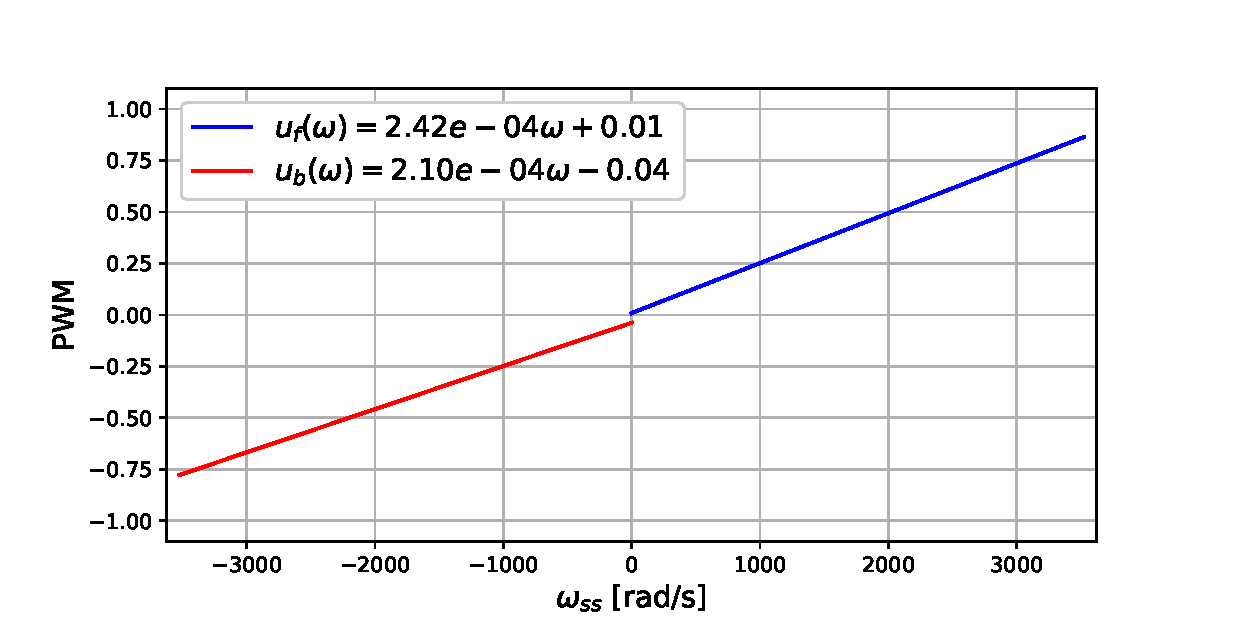
\includegraphics[width=\textwidth]{figuras/resultados/exp03/curva_feedforward_esquerdo100.eps}
    \caption{Curva $u(\omega)$ para o motor esquerdo.}
    \label{fig:exp03:curva_feedforward_esquerdo}
    \end{subfigure}
    \hfill
    \begin{subfigure}{.5\textwidth}
    \centering
    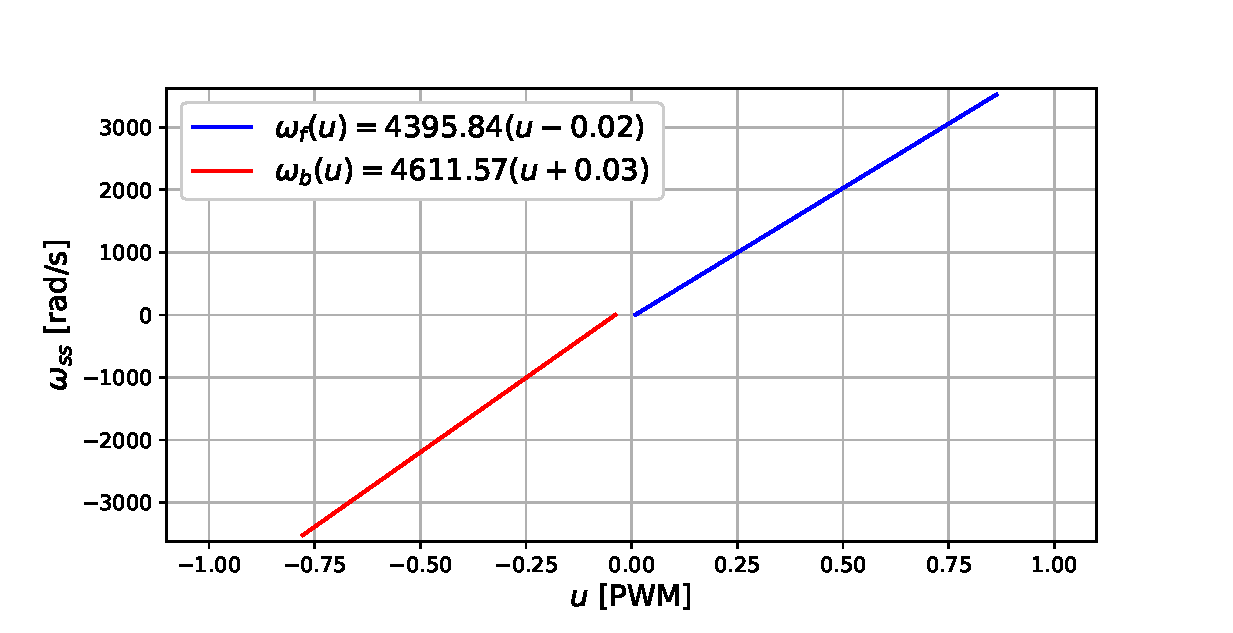
\includegraphics[width=\textwidth]{figuras/resultados/exp03/curva_feedforward_direito100.eps}
    \caption{Curva $u(\omega)$ para o motor direito.}
    \label{fig:exp03:curva_feedforward_direito}
    \end{subfigure}
    \begin{subfigure}{.5\textwidth}
    \centering
    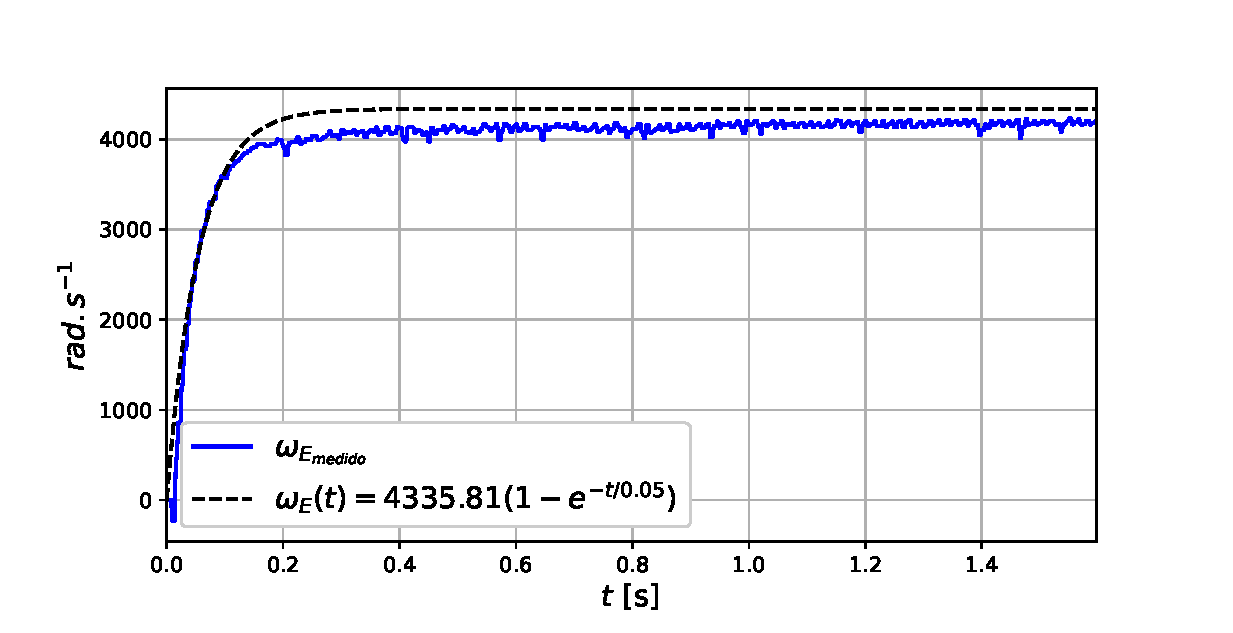
\includegraphics[width=\textwidth]{figuras/resultados/exp03/regressao_vs_medido_esquerdo100.eps}
    \caption{Curva $\omega(t)$ ideal, com os parâmetros da identificação vs velocidades medidas. Motor Esquerdo.}
    \label{fig:exp03:regressao_medido_esquerdo}
    \end{subfigure}
    \hfill
    \begin{subfigure}{.5\textwidth}
    \centering
    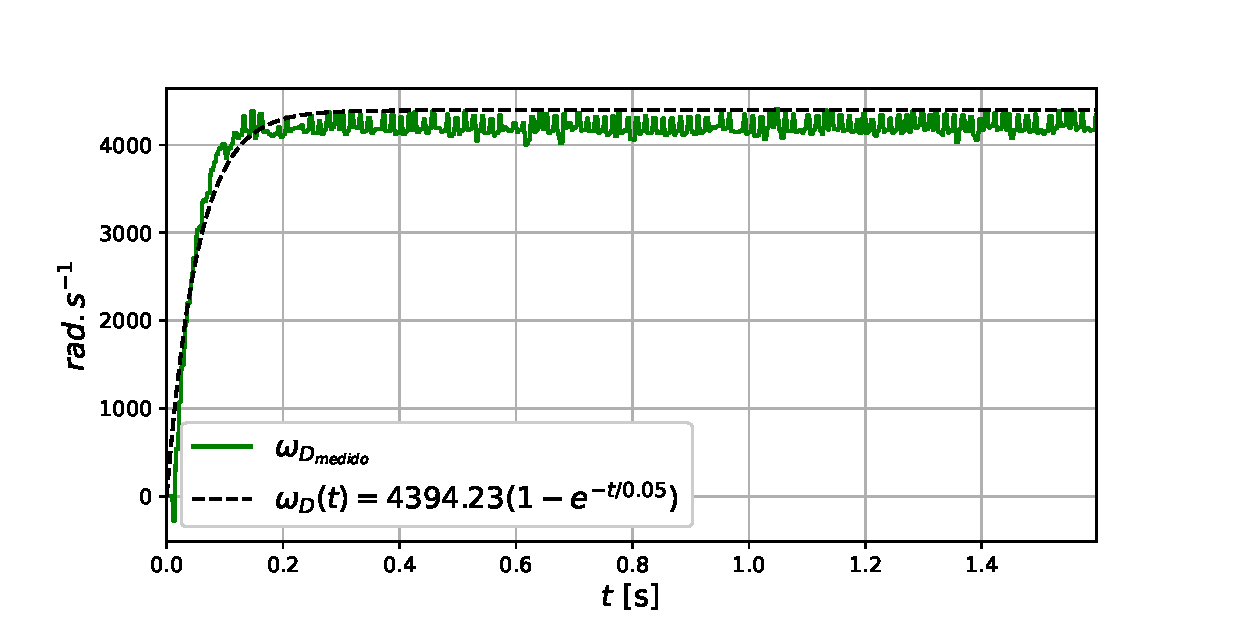
\includegraphics[width=\textwidth]{figuras/resultados/exp03/regressao_vs_medido_direito100.eps}
    \caption{Curva $\omega(t)$ ideal, com os parâmetros da identificação vs velocidades medidas. Motor Direito.}
    \label{fig:exp03:regressao_medido_direito}
    \end{subfigure}
    \hfill
    \begin{subfigure}{.5\textwidth}
    \centering
    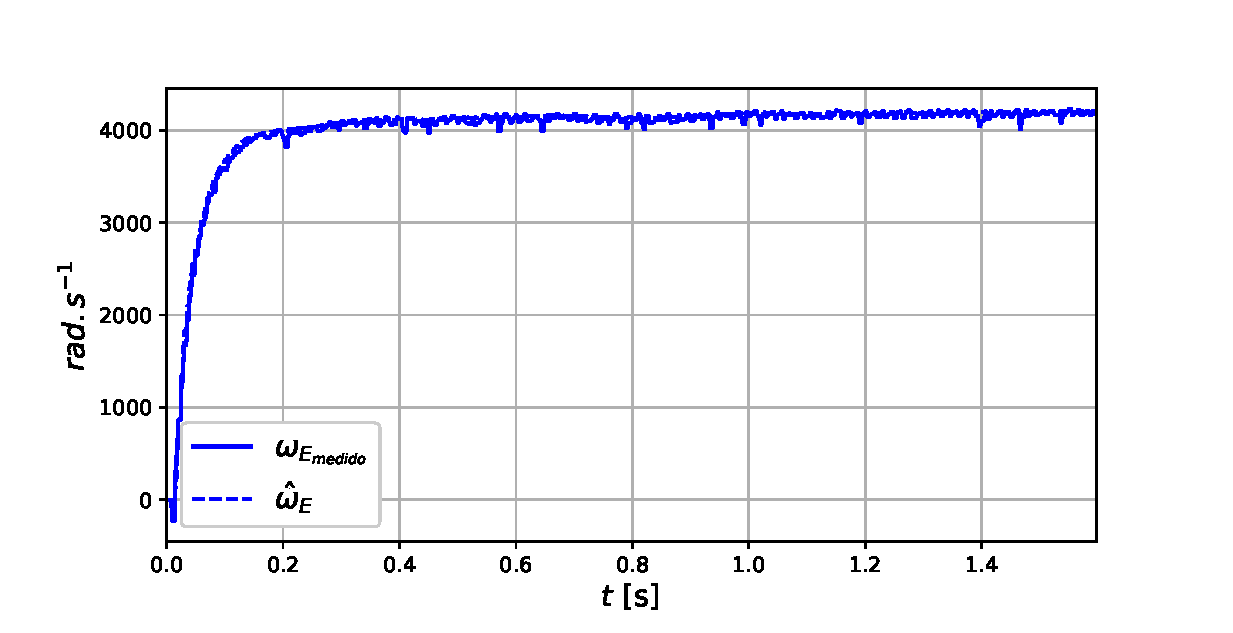
\includegraphics[width=\textwidth]{figuras/resultados/exp03/filtro_vs_sem_filtro_esquerdo100.eps}
    \caption{Comparação entre a velocidade estimativa $\hat{\omega}$ e a velocidade $\omega$ medida. Motor Esquerdo.}
    \label{fig:exp03:filtragem_esquerdo}
    \end{subfigure}
    \hfill
    \begin{subfigure}{.5\textwidth}
    \centering
    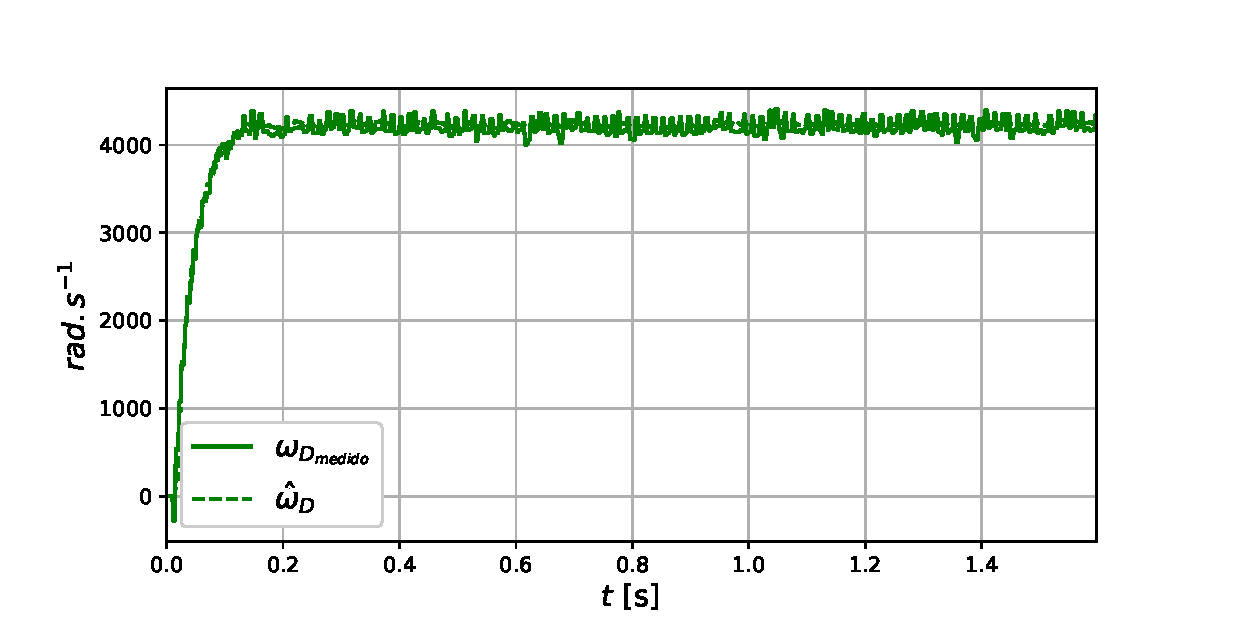
\includegraphics[width=\textwidth]{figuras/resultados/exp03/filtro_vs_sem_filtro_direito100.eps}
    \caption{Comparação entre a velocidade estimativa $\hat{\omega}$ e a velocidade $\omega$ medida. Motor Direito.}
    \label{fig:exp03:filtragem_direito}
    \end{subfigure}
    \hfill
    \begin{subfigure}{.5\textwidth}
    \centering
    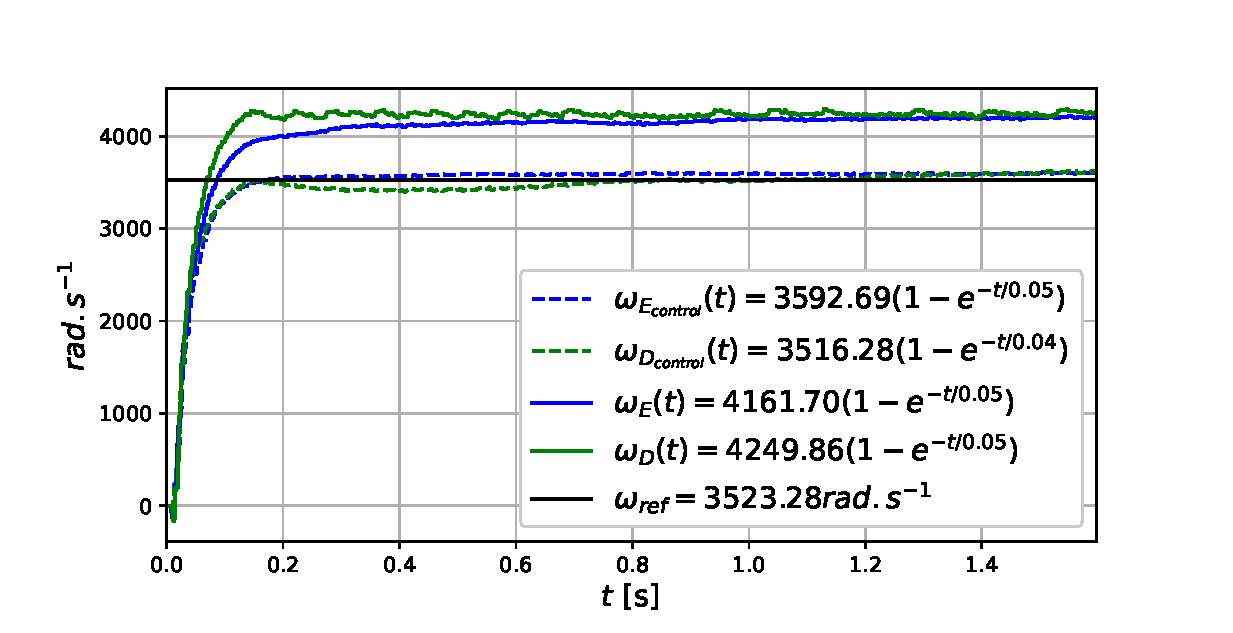
\includegraphics[width=\textwidth]{figuras/resultados/exp03/controlador_vs_sem_controlador100.eps}
    \caption{Comparação entre o sistema com controlador vs sem controlador.}
    \label{fig:exp03:controle}
    \end{subfigure}
    \hfill
    \begin{subfigure}{.5\textwidth}
    \centering
    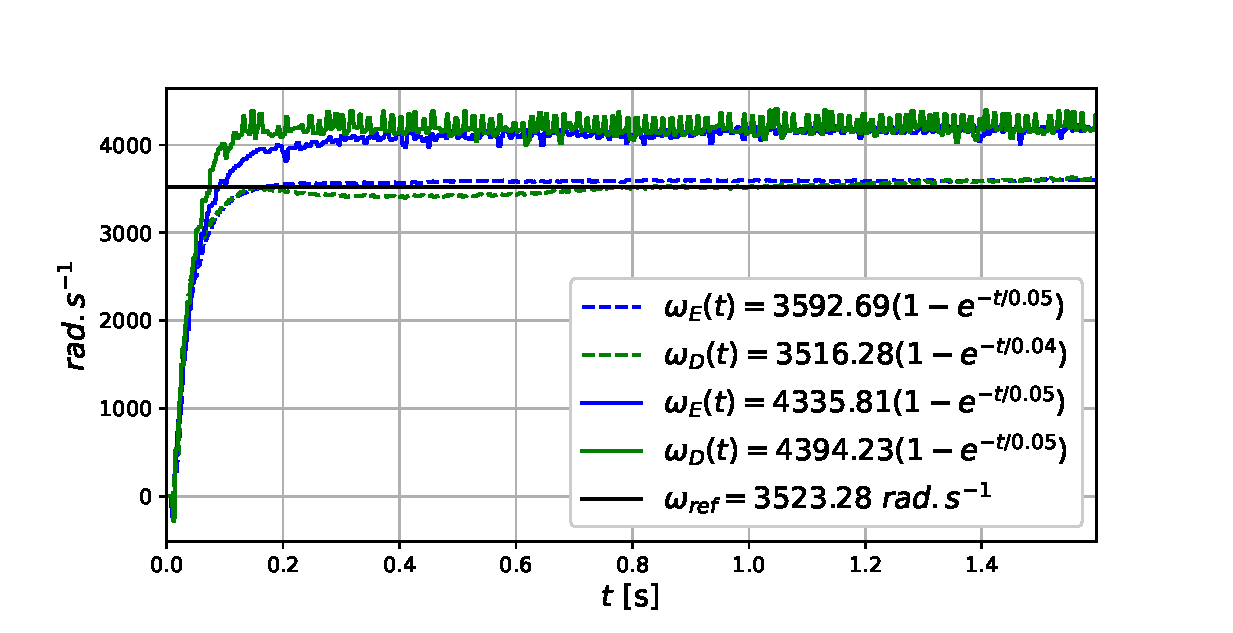
\includegraphics[width=\textwidth]{figuras/resultados/exp03/antes_vs_depois100.eps}
    \caption{Resposta sem observador e sem controle vs com controlador e observador.}
    \label{fig:exp03:antes_vs_depois}
    \end{subfigure}
    
    \caption{Experimento 3. \emph{Sinal de controle e Referência igual a 1.0.}}
    \label{fig:exp03_100}
\end{figure}

Os gráficos comparativos para o experimento 3 estão exibidos na Figura \ref{fig:exp03_100}. A partir dessas Figuras e da Tabela \ref{tab:resumo_calibracao} é possivel fazer as mesmas observações que no experimento 1 e 2, com a diferença nas zonas mortas (que podem ser observadas nas Figuras \ref{fig:exp03:curva_feedforward_esquerdo} e \ref{fig:exp03:curva_feedforward_direito}).


\begin{figure}[H]
    % \centering
    \begin{subfigure}{.5\textwidth}
    \centering
    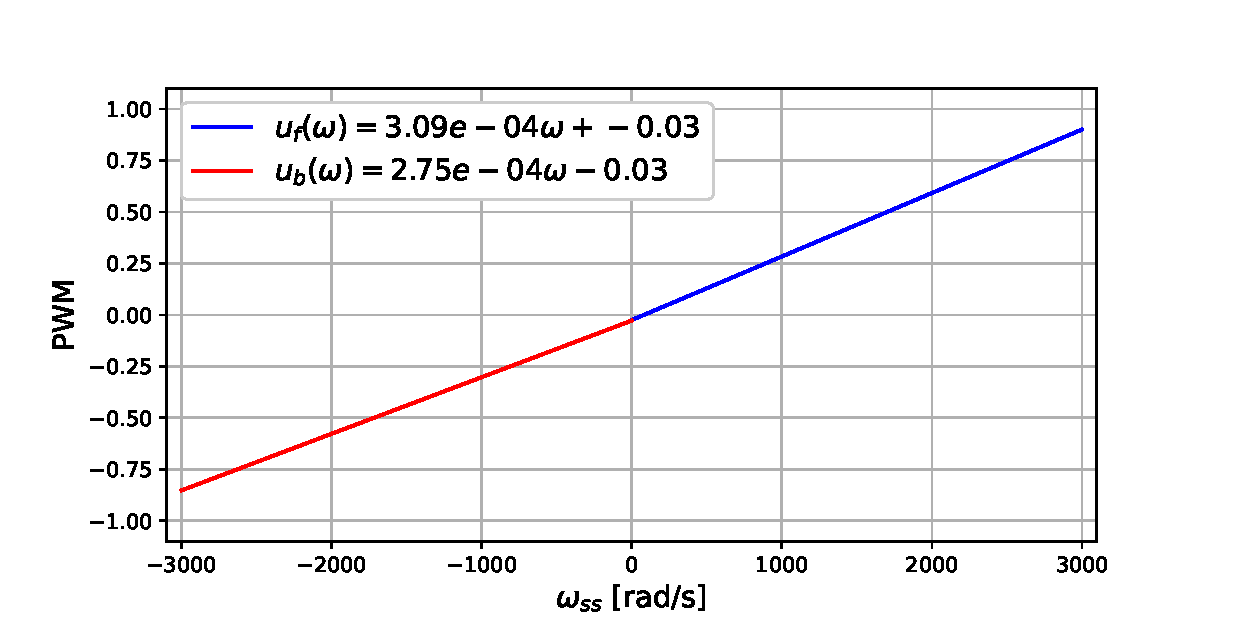
\includegraphics[width=\textwidth]{figuras/resultados/exp04/curva_feedforward_esquerdo100.eps}
    \caption{Curva $u(\omega)$ para o motor esquerdo.}
    \label{fig:exp04:curva_feedforward_esquerdo}
    \end{subfigure}
    \hfill
    \begin{subfigure}{.5\textwidth}
    \centering
    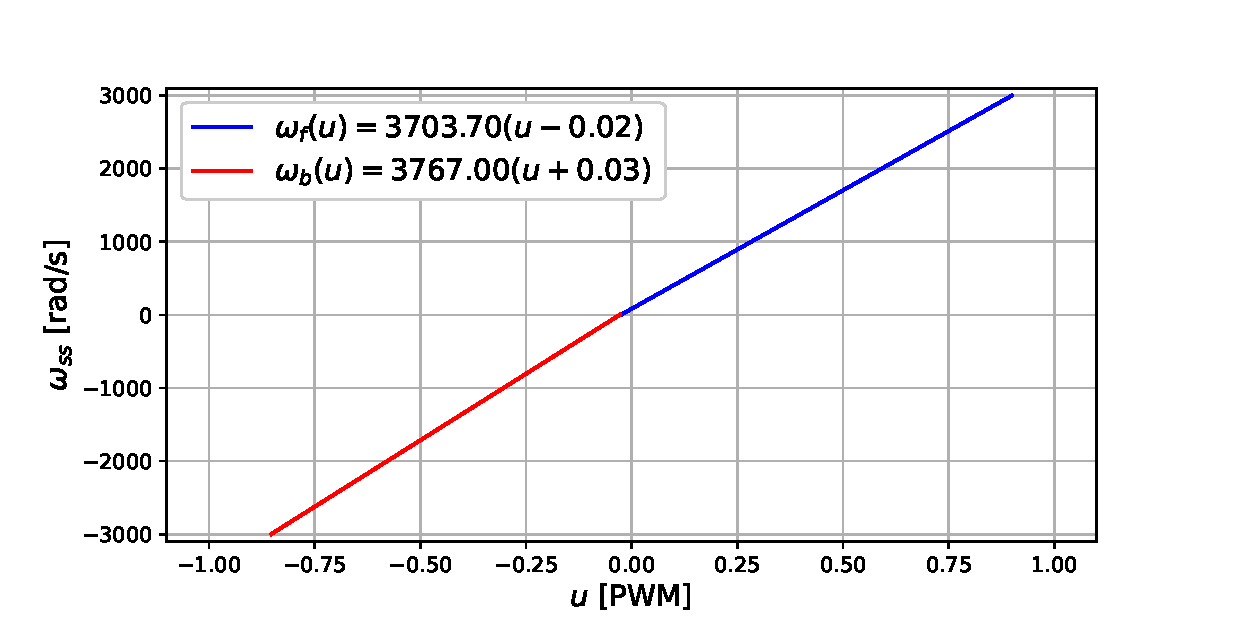
\includegraphics[width=\textwidth]{figuras/resultados/exp04/curva_feedforward_direito100.eps}
    \caption{Curva $u(\omega)$ para o motor direito.}
    \label{fig:exp04:curva_feedforward_direito}
    \end{subfigure}
    \begin{subfigure}{.5\textwidth}
    \centering
    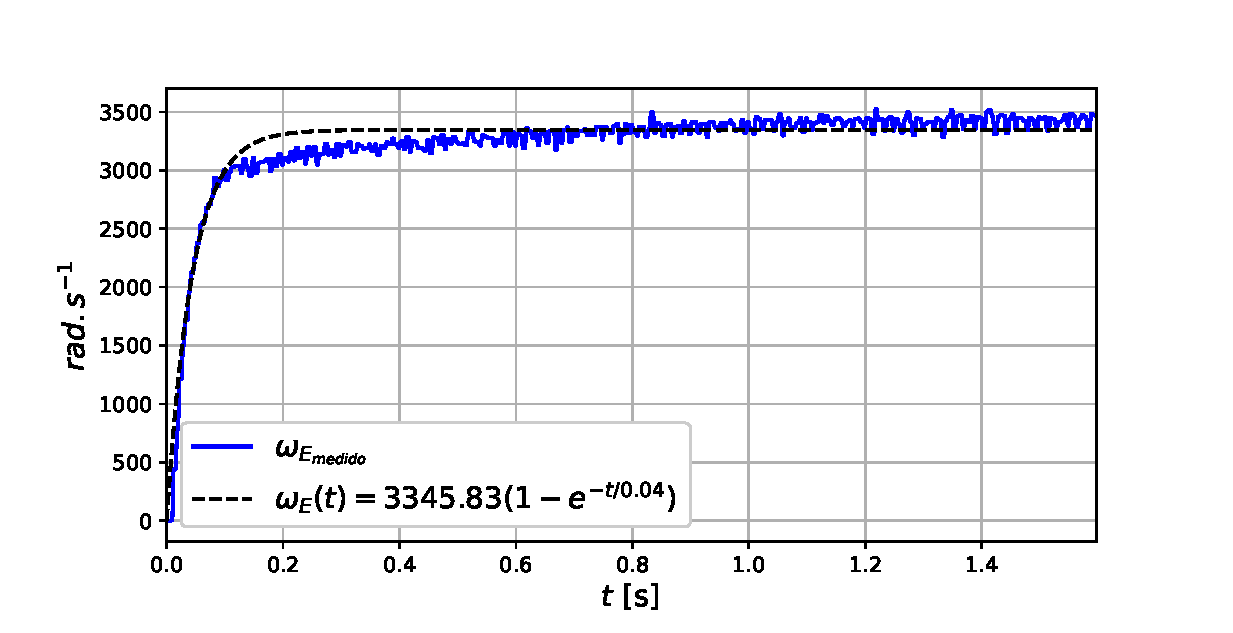
\includegraphics[width=\textwidth]{figuras/resultados/exp04/regressao_vs_medido_esquerdo100.eps}
    \caption{Curva $\omega(t)$ ideal, com os parâmetros da identificação vs velocidades medidas. Motor Esquerdo.}
    \label{fig:exp04:regressao_medido_esquerdo}
    \end{subfigure}
    \hfill
    \begin{subfigure}{.5\textwidth}
    \centering
    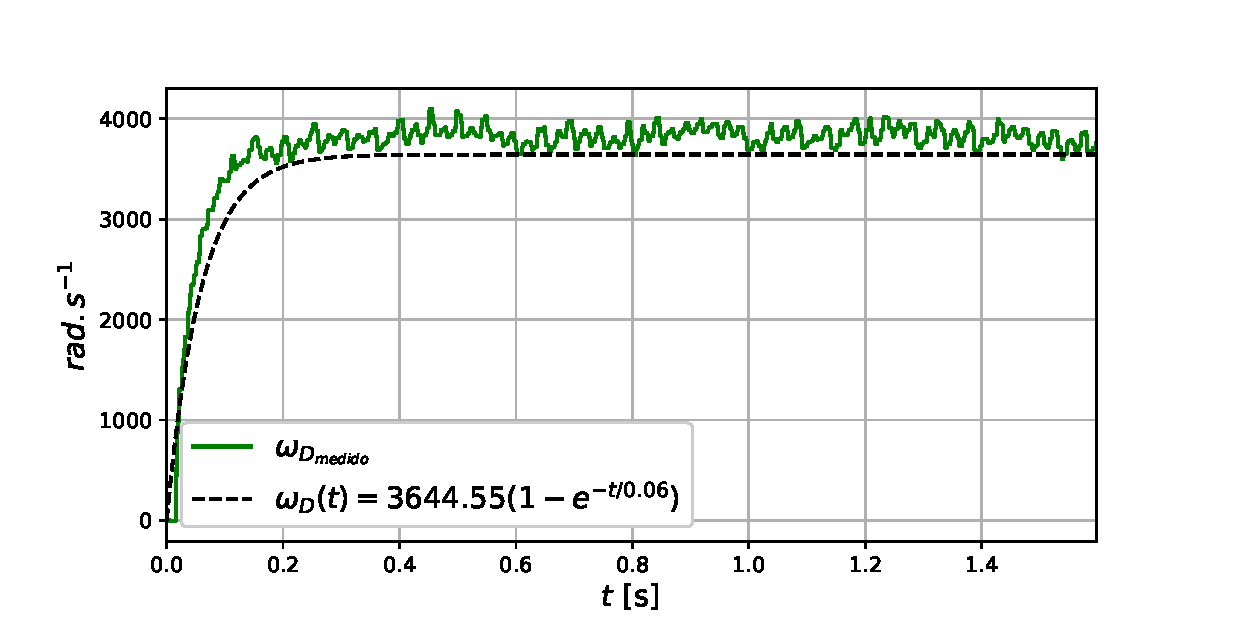
\includegraphics[width=\textwidth]{figuras/resultados/exp04/regressao_vs_medido_direito100.eps}
    \caption{Curva $\omega(t)$ ideal, com os parâmetros da identificação vs velocidades medidas. Motor Direito.}
    \label{fig:exp04:regressao_medido_direito}
    \end{subfigure}
    \hfill
    \begin{subfigure}{.5\textwidth}
    \centering
    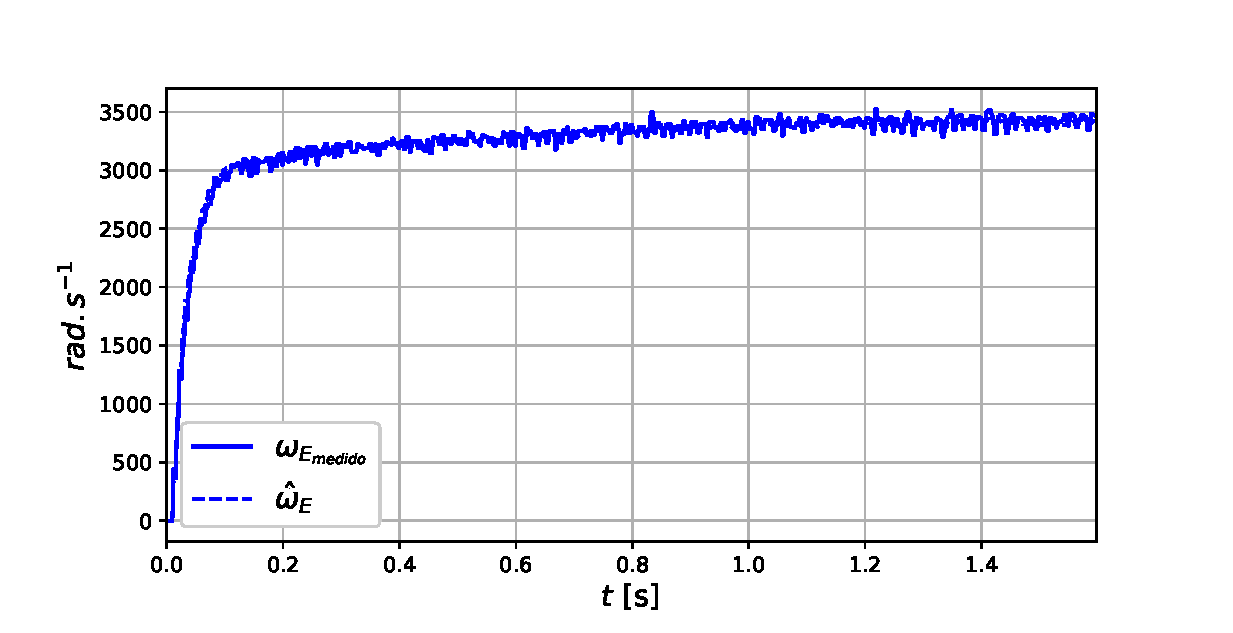
\includegraphics[width=\textwidth]{figuras/resultados/exp04/filtro_vs_sem_filtro_esquerdo100.eps}
    \caption{Comparação entre a velocidade estimativa $\hat{\omega}$ e a velocidade $\omega$ medida. Motor Esquerdo.}
    \label{fig:exp04:filtragem_esquerdo}
    \end{subfigure}
    \hfill
    \begin{subfigure}{.5\textwidth}
    \centering
    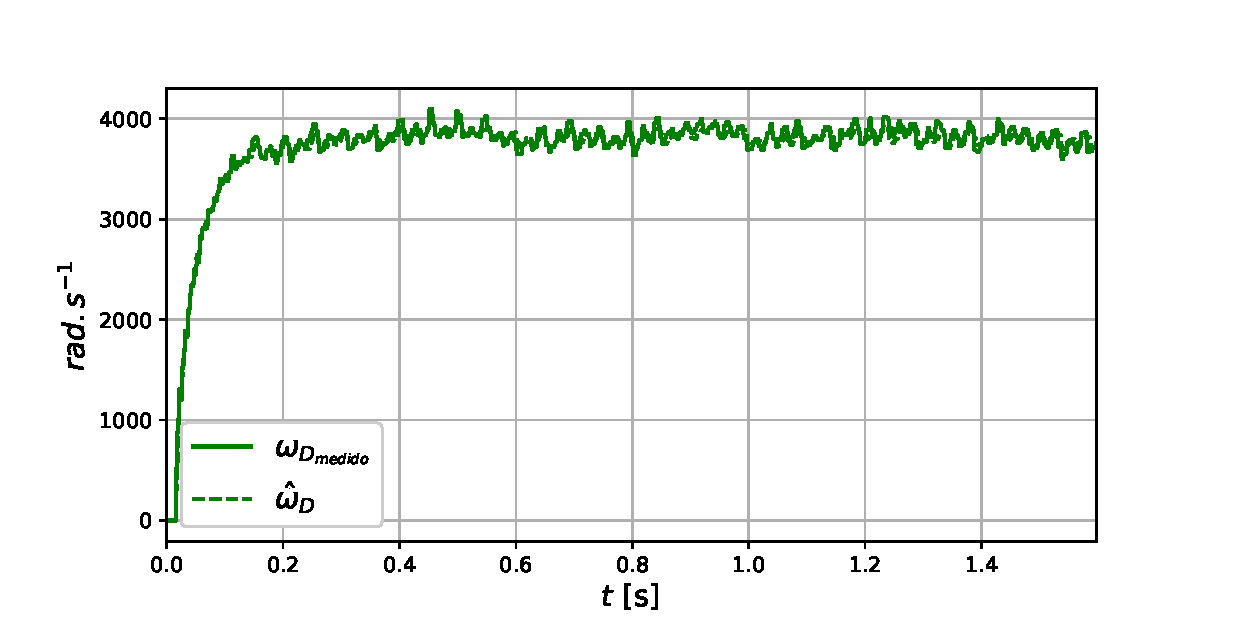
\includegraphics[width=\textwidth]{figuras/resultados/exp04/filtro_vs_sem_filtro_direito100.eps}
    \caption{Comparação entre a velocidade estimativa $\hat{\omega}$ e a velocidade $\omega$ medida. Motor Direito.}
    \label{fig:exp04:filtragem_direito}
    \end{subfigure}
    \hfill
    \begin{subfigure}{.5\textwidth}
    \centering
    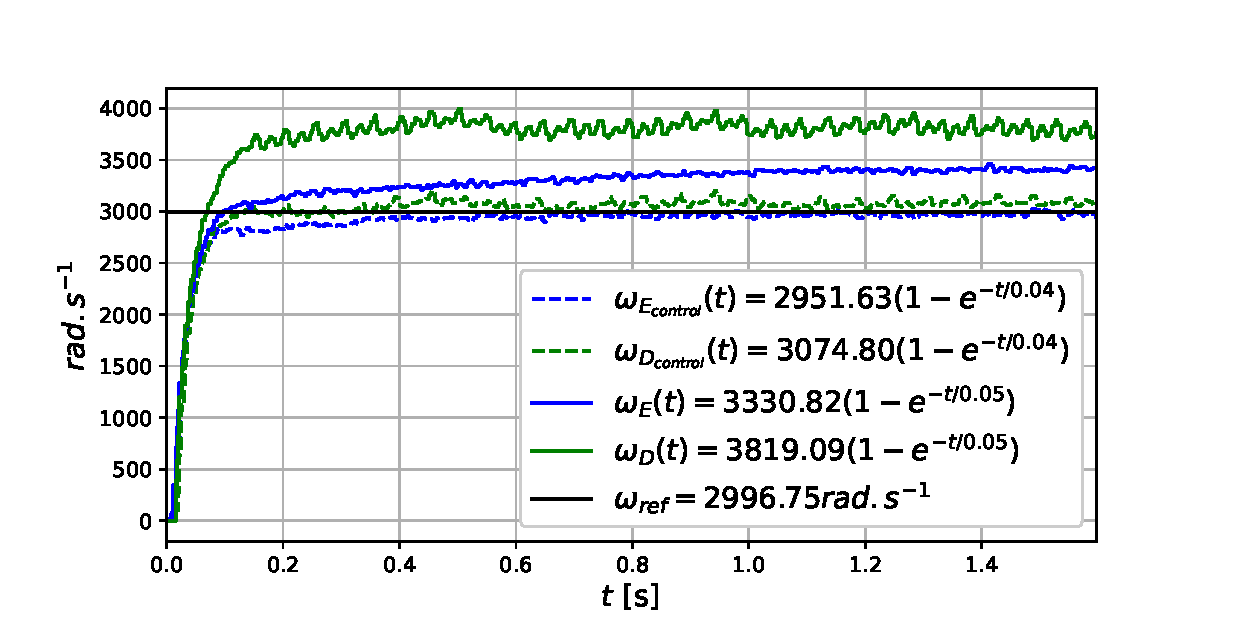
\includegraphics[width=\textwidth]{figuras/resultados/exp04/controlador_vs_sem_controlador100.eps}
    \caption{Comparação entre o sistema com controlador vs sem controlador.}
    \label{fig:exp04:controle}
    \end{subfigure}
    \hfill
    \begin{subfigure}{.5\textwidth}
    \centering
    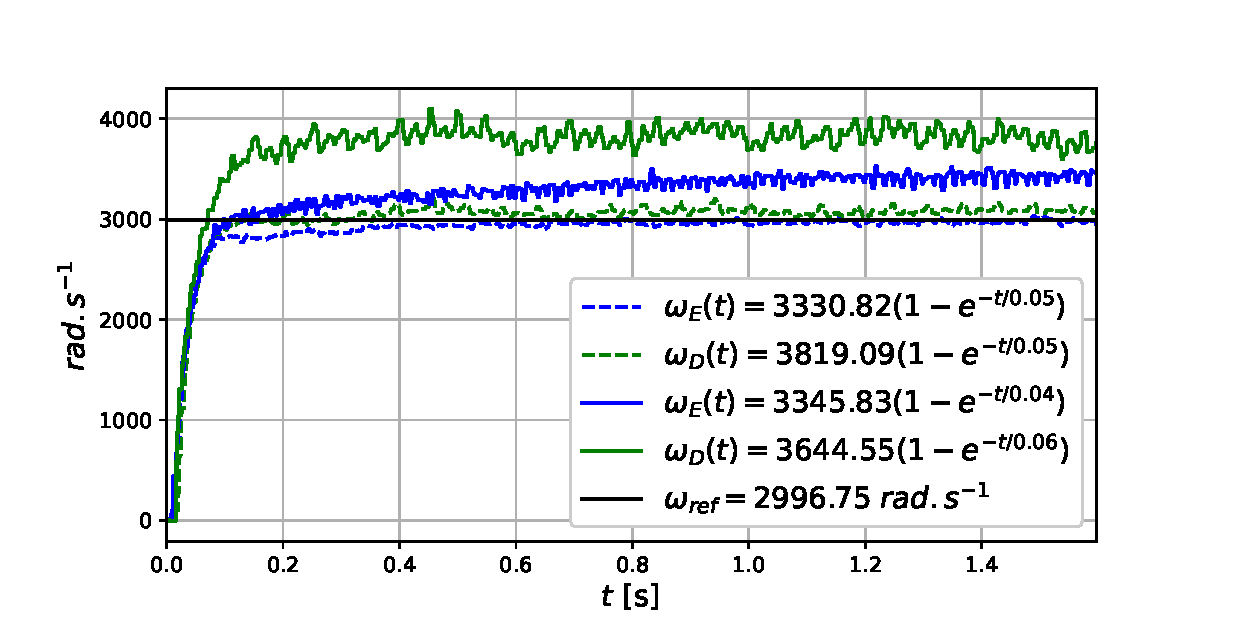
\includegraphics[width=\textwidth]{figuras/resultados/exp04/antes_vs_depois100.eps}
    \caption{Resposta sem observador e sem controle vs com controlador e observador.}
    \label{fig:exp04:antes_vs_depois}
    \end{subfigure}
    
    \caption{Experimento 4. \emph{Sinal de controle e Referência igual a 1.0.}}
    \label{fig:exp04_100}
\end{figure}

Os gráficos comparativos para o experimento 4 estão exibidos na Figura \ref{fig:exp04_100}. A partir dessas Figuras e da Tabela \ref{tab:resumo_calibracao} extraí-se que para o \textbf{Experimento 4}:

\begin{itemize}
    \item Analisando as Figuras \ref{fig:exp04:curva_feedforward_esquerdo} e \ref{fig:exp04:curva_feedforward_direito}:\\
        As zonas mortas ($|D|$) para o motor esquerdo e direito são respectivamente: $0.03$ (para ambos os sentidos de giro), $0.02$ e $0.03$ (na rotação que favorece o movimento para frente do robô e para trás, respectivamente).
    \item Pelas Figuras \ref{fig:exp04:regressao_medido_esquerdo} e \ref{fig:exp04:regressao_medido_direito}:\\
        Observa-se que, as curvas ideais/teóricas (considerando o sistema de primeira ordem e com os parâmetros da calibração) conseguem representar bem o comportamento apresentado pela resposta dos motores esquerdo e direito.
    \item Pelos gráficos das Figuras \ref{fig:exp04:filtragem_esquerdo} e \ref{fig:exp04:filtragem_direito} observa-se que:\\
        para ambos os motores a curva correspondente à velocidade $\hat{\omega}$ estimada pelo filtro, encontra-se sobrepondo-se a curva das velocidades medidas, porém, com um ruído bem menor.
    \item Já pela Figura \ref{fig:exp04:controle} nota-se para ambos os motores:
        Que a resposta do sistema controlado está bem próximo da referência $\omega_{ref}$ e que a constante de tempo $\tau$ está como o desejado ($0.05s$).
    \item Por fim a Figura \ref{fig:exp04:antes_vs_depois} compara a resposta do sistema com o controlador+observador, com os mesmos sem estes. \\
        Nota-se que os conjuntos motor-roda esquerdo e direito apresentam assimetrias significativas, principalmente com relação ao  ganho (o conjunto direito apresenta-se com um ganho maior). Porém a resposta controlada mostrou que se conseguiu diminuir significativamente essas assimetrias nesse experimento.
\end{itemize}